\section{Аналитический метод}

\begin{theorem}\label{th1}
Вполне смешанная игра $(m \times n)$-игра $\Gamma$ имеет единственную ситуацию равновесия
$(x^*, y^*)$ и квадратную матрицу $(m = n)$; если цена игры $v \neq 0$, то матрица $C$
невырожденная и

\begin{equation}\label{f1}
    x^* = \frac{uC^{-1}}{uC^{-1}u^T}, \quad y^* = \frac{C^{-1}u^T}{uC^{-1}u^T}, \quad v = \frac{1}{uC^{-1}u^T},
\end{equation}

где вектор $u = (1, 1, \dots, 1) \in \mathbb{R}^m$.

\end{theorem}

Используя теорему~\ref{th1}, посчитаем цену игры и стратегии для обоих игроков согласно
формулам~\ref{f1}.

Вывод программы с посчитанным результатом приведен на рисунке~\ref{fig:fig02}.

\begin{figure}
  \centering
  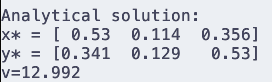
\includegraphics[scale=0.7]{../../artifacts/lw1/analytical_solution.png}
  \caption{Ответ для задачи, посчитанный аналитическим методом}
  \label{fig:fig02}
\end{figure}

Далее решим игру численным методом Брауна--Робинсон.
